\chapter{Experiments and Evaluation Metrics}

In this chapter we will go over the various experiments and metrics used to evaluate the performance of our methods. This information is subsequently divided into three sections.

In the first section we will show the metrics used to describe the performance of the pose estimation network. In the second section we will then show how we evaluated the performance of our semantic meaning extraction strategy. Finally, in the third section we will discuss the experimental setup we used to test the performance of our complete model in a real-life robotics application.

\section{Evaluation Metrics for Pose Esitmation and Object Detection}

Most pose estimation and object detection methods share a common set of metrics on which their performance is evaluated. These are namely Average Precision for object detection strategies, and Average Distance and ADD for pose estimation strategies. In this section we will describe each metric, its meaning and how it is computed.

\subsection{Average Precision}

The performance of object detectors and 2D bounding box regressors is usually evaluated using Average Precision (AP), which is a descriptor of the reliability of a method's predictions. It exploits the intersection over union (IoU), computed as:

\begin{equation*}
    \text{IoU} = \frac{B_{GT} \cap B_{P}}{B_{GT} \cup B_{P}}
    \label{eq:IoU}
\end{equation*}

where $B_{GT}$ is the area of the ground truth bounding box and $B_{P}$ is the area of the network's predicion. A prediction is considered true if its IoU is greater than a \emph{threshold}; based on this, we can generate the model's confusion matrix, as described in table \ref{confusionmatrix}.

\begin{table}[ht]
    \begin{center}
        \begin{tabular}{c||c|c}
            \space & Actual Positives & Actual Negatives\\
            \hline\hline
            Predicted Positives & True Positives (TP)& False Positives (FP)\\
            \hline
            Predicted Negatives & False Negatives (FN)& True Negatives (TN)\\
        \end{tabular}
        \caption{Generation of the confusion matrix.}
        \label{confusionmatrix}
    \end{center}
\end{table}

This matrix is the basis for the definition of the precision and recall metrics. Precision is an indicator of how well the model avoids false positives, while recall is an indicator of how well a model avoids false negatives. They are computed as follows:

\begin{align*}
    \text{Precision (P)} &= \frac{\text{TP}}{\text{TP} + \text{FP}}\\
    \text{Recall (R)} &= \frac{\text{TP}}{\text{TP} + \text{FN}}
\end{align*}

Precision and recall both depend on the value of the IoU \emph{threshold}: larger values will result in a more restrictive model, thus less false positives and more false negatives, high precision and low recall, while smaller values will result in the opposite: more false positives, less false negatives, low precision and high recall.

It is common practice to plot the precision as a function of the recall in what is called a precision-recall curve, $P = f(R)$. Each point in the curve represents a value of the \emph{threshold}, corresponding to its own confusion matrix and subsequent precision and recall metrics. An example plot is shown in figure \ref{example_pr}.

\begin{figure}[ht]
    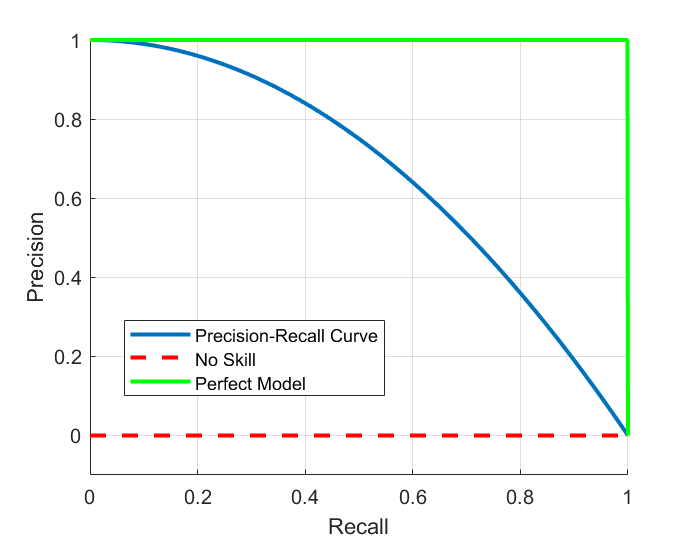
\includegraphics[width=0.6\textwidth]{example_pr_curve.png}
    \caption{Example of precision recall curves. The red line indicates a no-skill model with zero precision; the blue line a model with some skill; the green line is the ideal behavior with maximum precision and recall at all times.}
    \label{example_pr}
\end{figure}

At this point we can describe the Average Precision (AP) as the mean value of the precision, corresponding to the area under the precision-recall curve:

\begin{equation*}
    \text{AP} = \int_{0}^{1} f(R)dR
\end{equation*}

Therefore it is a real value between 0 and 1, with 0 representing the model with zero precision, and 1 representing the ideal behavior.

\subsection{Average Distance and ADD}
\label{add_description}

Evaluation of pose estimation methods is almost exclusively done using the ADD metric, and by extension the Average Distance (AD). While the first is an indicator of the percentage of correct estimations, similar in a sense to mAP, the second is instead unique to pose estimation.

Given $n$ points belonging to the 3D model $M$ of an object, the AD represents the average of the distance between these points transformed according to the ground truth ($\text{R}, \text{t}$) and according to the prediction ($\hat{\text{R}}, \hat{\text{t}}$):

\begin{equation*}
    \text{AD} = \frac{1}{n} \sum_{x \in M} ||(\text{R}x + \text{t}) - 
    (\hat{\text{R}}x + \hat{\text{t}})||_2
\end{equation*}

The ADD is then given by the percentage of correct poses given by the model. A pose is correct if its AD metric is less than 10\% of the 3D model's diameter.

This metric has serious issues when dealing with objects that have rotational symmetries, as these objects present no visual differences for multiple different orientations. For example, one image of the M6x30 screw we use for inferencing could correspond to six different poses, each varying 60\degree from the previous one. This means that the model will eventually stabilize at a value that minimizes the average error, which is ususally large.

To combat this issue, we use the Symmetric Average Distance (AD-S)\cite{PoseCNN} metric, defined as the average minimum distance between points in the predicted pose and the ground truth:

\begin{equation*}
    \text{AD-S} = \frac{1}{n} \sum_{x_1 \in M} \min_{x_2 \in M} ||(\text{R}x_2 + \text{t}) - 
    (\hat{\text{R}}x_1 + \hat{\text{t}})||_2
\end{equation*}

This considers the distance from each point to its closest correspodent in the ground truth. Analogously to ADD, we then implement ADD-S as the percentage of correct poses.

We would like our model to obatin the highest possible ADD-S, however in an industrial environment it is important to also evaluate the AD. This is because for larger objects the ADD will tolerate greater estimation errors, as it is based on the diameter of the objects; these errors however may not be compatible with the precision required for a determined task.

\section{Semantics Evaluation Methodology}
\label{semantics_method_section}

To evaluate our semantic meaning extraction method, we must compare ground truth values for the semantic state of each scene, associated with its own image, with the outputs of our method.

Our strategy therefore is to save the semantic state for each image during dataset generation as the ground truth. We then run the trained model on the test dataset to obtain pose and class predictions, use these results to run our semantic meaning extraction method, and evaluate the results against the ground truth. In particular we select a button-slot \emph{distance metric} and \emph{distance threshold} for each experiment, and compare the estimate of the state of each slot, for each board in each scene, against its true value.

However, an issue arises from this application: due to the symmetry of the boards, it is impossible to determine visually which slot is which. For example in figure \ref{sym_eval}, the ground truth is that there is a button in the first slot and the second slot is empty, however, the model may output that the button is in the second slot, while the first slot is empty. Visually, both of these interpretations are correct, since the board is symmetrical, but directly comparing the prediction with the ground truth results in two "false" values: a false negative for the first slot and a false positive for the second, resulting in an untrue evaluation.

\begin{figure}[ht]
    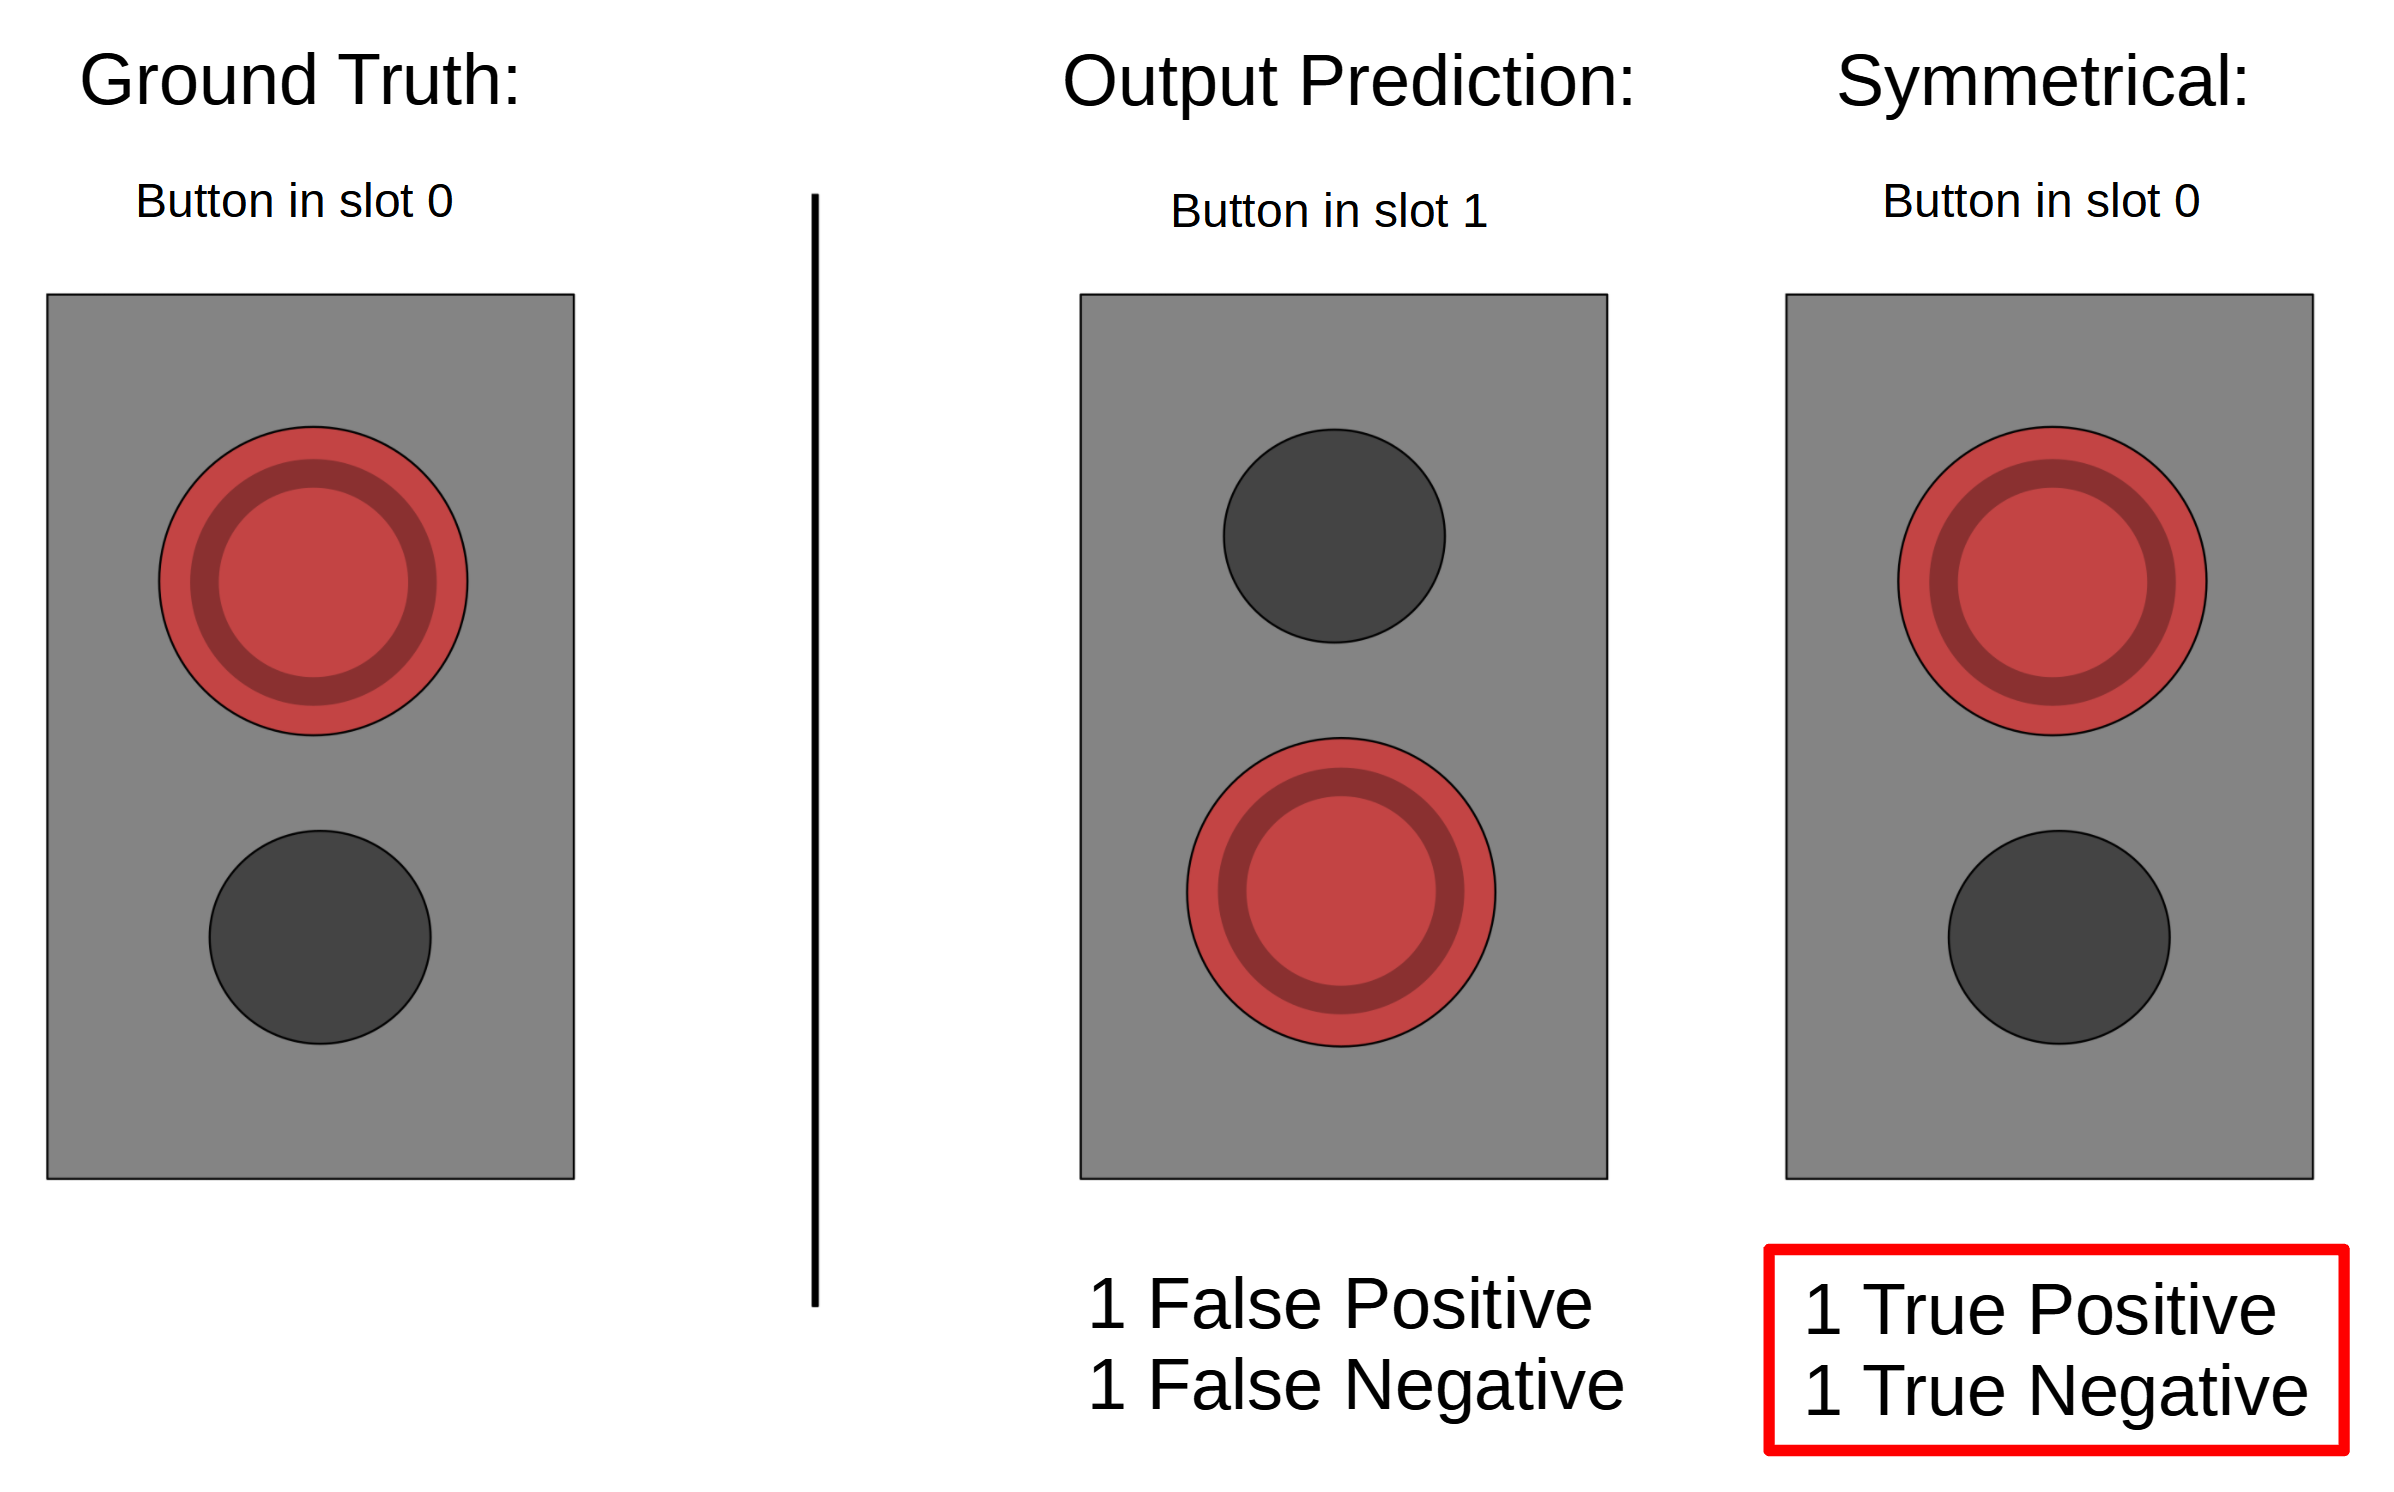
\includegraphics[width=0.8\textwidth]{sym_evaluation.png}
    \caption{Schematic depiction of a board with a button slotted into the first slot. The model runs into issues because the prediction and its symmetrical are visually undistinguishable and give different results.}
    \label{sym_eval}
\end{figure}

To combat this issue, for each board we take into account both the model's prediction, and its symmetrical, obtained by simply reversing the order of its slots. For the example in figure \ref{sym_eval}, the prediction is [empty, button], therefore its symmetrical is [button, empty]. We then only consider the results from the version with the greatest number of "true" values when compared with the ground truth. For the example, since the symmetrical results in two "true" values, the final output of the comparison is two "true" values: a true positive and a true negative. These values are then summed for all estimations computed using a determined \emph{distance metric} and \emph{distance threshold}, and the sums are used to build a confusion matrix. Thus by evaluating a variety of \emph{distance thresholds}, we can build a precision-recall curve as described in the previous section.

The selection of the optimal \emph{distance threshold} is done by considering the F1 score: a balanced function of precision and recall, computed as:

\begin{equation*}
    \text{F1} = 2\times\frac{\text{Precision}\times\text{Recall}}{\text{Precision}+\text{Recall}}
\end{equation*}

We consider the optimal threshold to be the one that maximises this value.

\section{Real-Life Experimental Setup}

To test the effectiveness of our vision and semantics model, we implemented it in a real life situation where we have to complete a simple assembly task. We used a Doosan A0509s robotic manipulator equipped with a pneumatic gripper, and an Azure Kinect camera. We then re-implemented previously developed code for this system that generates behavior trees \cite{behavior_tree} to drive the robot based on previous demostrations of actions and their effects on the scene.

Our contribution is mostly in the perception phase of this architecture, where we perform three tasks:

\begin{enumerate}
    \item From the RGB image provided by the camera, detecting objects of interest and estimating their position.
    \item Understanding the state of the interactions between the detected objects.
    \item Building a list of predicates that describes the scene.
\end{enumerate}

\begin{figure}[ht]
    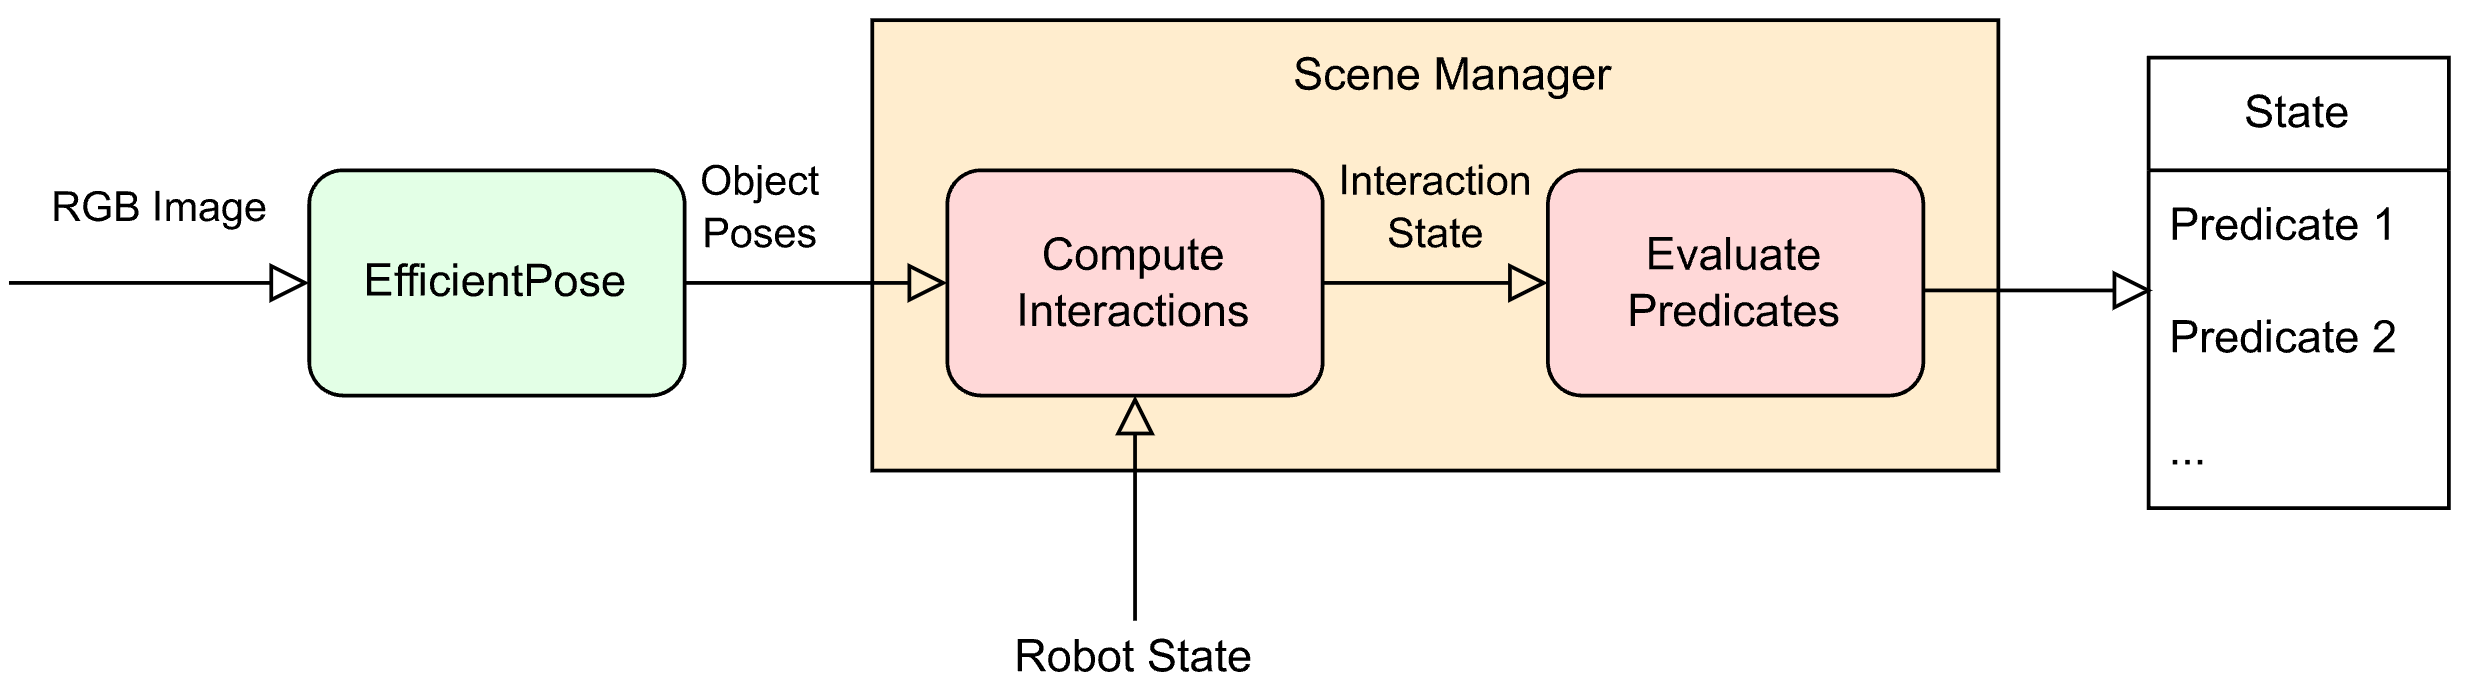
\includegraphics[width=\textwidth]{vision_system.png}
    \caption{Schematic representation of the overall vision system.}
\end{figure}

While the first step is performed by the network, the final two are performed by what is known as the Scene Manager. The ultimate objective of the Scene Manager is to describe a scene using a set of predicates: first-order logic functions that can be either true or false. Their value is updated for each object whenever we obtain new information on the scene, with the ones resulting true then being compiled into the \emph{state}. For our application, this is accomplished using the predicates in table \ref{predicateslist}.

\begin{table}[ht]
    \begin{center}
        \resizebox{0.9\columnwidth}{!}{
            \begin{tabular}{cc}
                Predicate & Description \\
                \hline \hline
                IsGripperEmpty(gripper) & True when no objects are in the gripper. \\
                \hline
                IsGrasped(button, gripper) & True when the button is grasped by the gripper. \\
                \hline
                IsButtonInSlot(button, slot) & True when the button is inserted in the slot. \\
                \hline
                IsSlotEmpty(slot) & True when no buttons are in the slot.\\
            \end{tabular}
        }
        \caption{List of predicates used to describe the state in our application.}
        \label{predicateslist}
    \end{center}
\end{table}

\begin{figure}[ht]
    \includegraphics[width=\textwidth]{actions_states.png}
    \caption{Evolution of the state and actions for the example task of picking up a button and inserting it into a slot.}
    \label{predicatesevolutions}
\end{figure}

The experiments with the robot consist of two phases: \emph{teaching mode} or \emph{evaluation mode}.

In \emph{teaching mode}, we show the robot how to perform actions through kinesthetic demostrations. During these demostrations, the robot, moved by a human operator, will modify the environment and thus change the scene. The actions performed during this phase, can be divided into move actions and interactions, which in our case are limited to opening and closing the gripper. Move actions reference a destination position, which we save relative to a manually defined reference object. For example, if we want to pick up a button, we set the reference to the button itself: this way when we require repeating the same actions but the button is in a different position, we can compute the new position by changing the initial reference pose, so as to not lose in generality.

\begin{figure}
    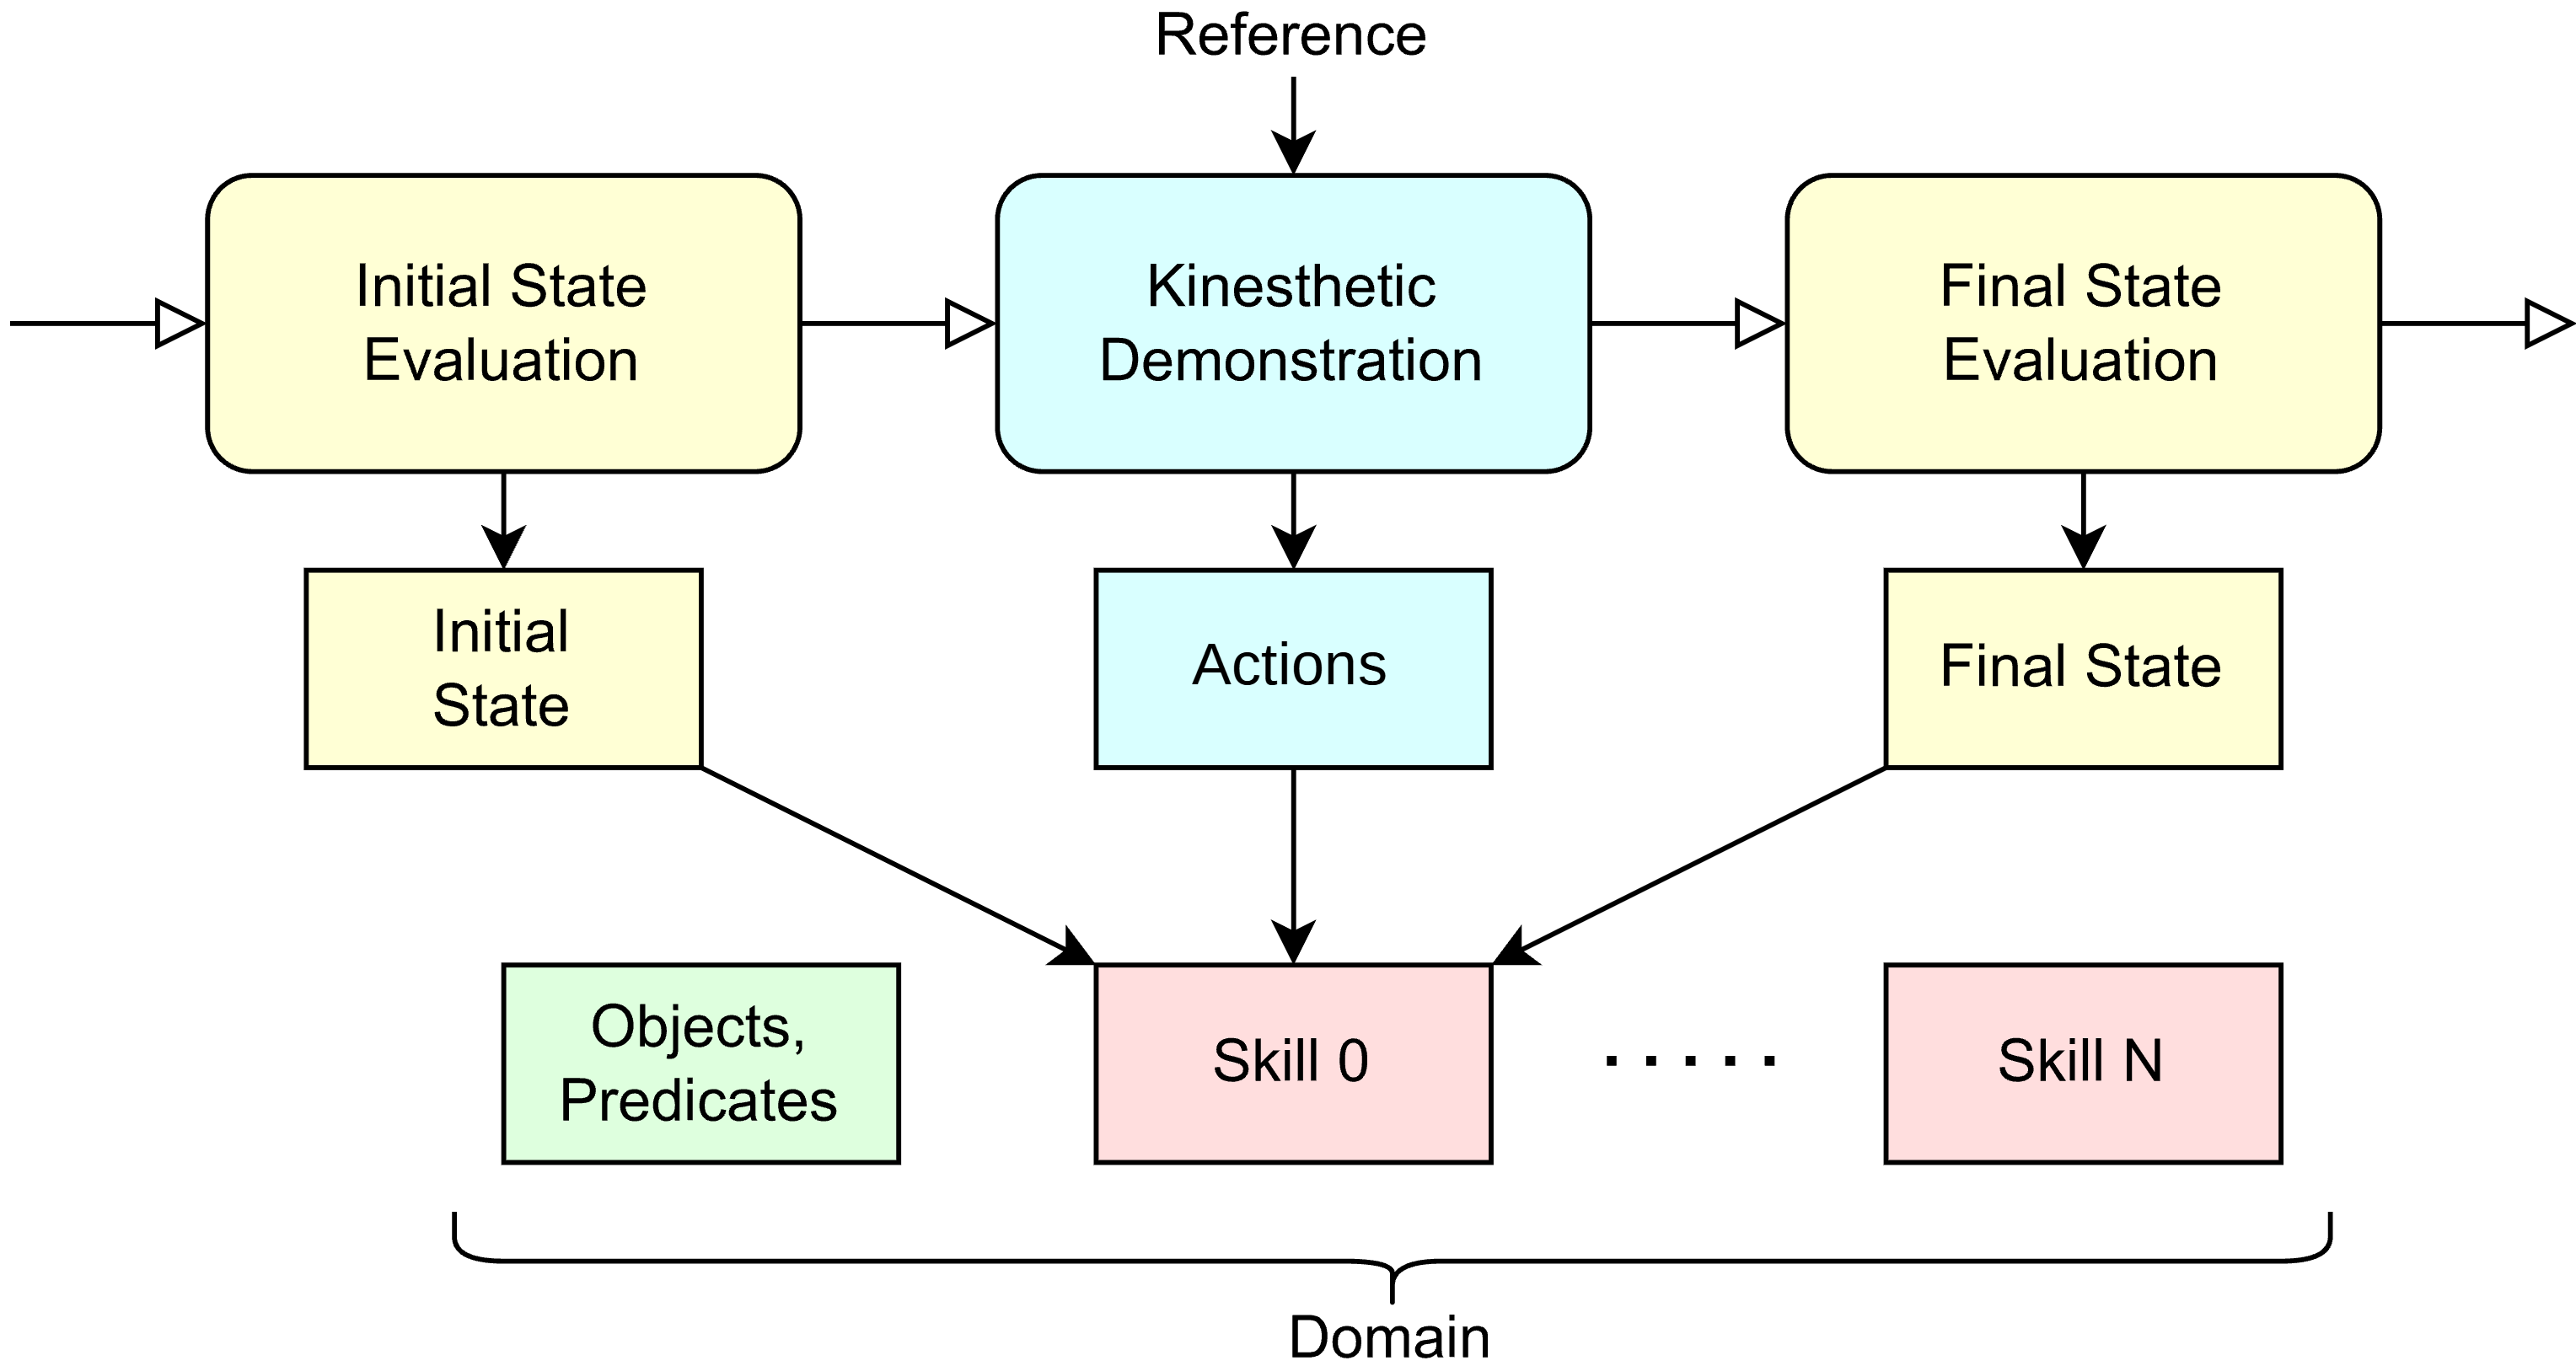
\includegraphics[width=0.9\textwidth]{teaching_mode.png}
    \caption{Schematic representation of phases and data flow in teaching mode.}
\end{figure}

By examining the differences between the state before and after the demonstration, we can use Planning Domain Definition Language (PDDL) \cite{pddl} to generate a set of \emph{preconditions} and \emph{effects} expressed in predicate form, and combine them with the low level robotic actions to obtain a \emph{skill}. For our example case shown in figure \ref{predicatesevolutions}, we define two \emph{skills} as shown below. The \emph{domain} for this task then consists of the set of all defined predicates and actions.

In \emph{evaluation mode} we specify what is known as the \emph{problem}. This consists of a combination of the semantic meaning of the scene's initial state (\emph{init}) and the final state we would like to achieve (\emph{goal}). By providing a PDDL planner with a \emph{domain} and \emph{problem}, it will compute the ordered set of actions necessary to pass from the initial to the final states described in the problem.

A behavior tree is then built by combining the individual trees for each action, in the order defined by the planner. These trees, united with our prior modelling of the task in the form of the domain and the problem, form a \emph{knowledge base} that is fundamental for the task's execution. Tthe robot's actions are then performed by evaluating the tree.

\begin{minipage}[t]{0.5\textwidth}
    \begin{lstlisting}[language=PDDL]
(:action action_0
    :parameters(
        ?Gripper1 - Gripper
        ?SmallButton1 - SmallButton
    );end_of_parameter
    :precondition (and
        (is_gripper_empty ?Gripper1)
    );end_of_precondition
    :effect (and
        (is_grasped ?SmallButton1 ?Gripper1)
        (not (is_gripper_empty ?Gripper1))
        (increase (total-cost) 50)
    );end_of_effect
);end_of_action
    \end{lstlisting}
\end{minipage}
\hfill
\begin{minipage}[t]{0.5\textwidth}
    \begin{lstlisting}[language=PDDL]
(:action action_1
    :parameters(
        ?SmallButton1 - SmallButton
        ?Gripper1 - Gripper
        ?Slot1 - Slot
    );end_of_parameter
    :precondition (and
        (is_grasped ?SmallButton1 ?Gripper1)
        (is_slot_empty ?Slot1)
    );end_of_precondition
    :effect (and
        (is_gripper_empty ?Gripper1)
        (is_button_in_slot ?SmallButton1 ?Slot1)
        (not (is_grasped ?SmallButton1 ?Gripper1))
        (not (is_slot_empty ?Slot1))
        (increase (total-cost) 50)
    );end_of_effect
);end_of_action 
    \end{lstlisting}
\end{minipage}

\begin{wrapfigure}{r}{0.4\textwidth}
    \centering
    \includegraphics[width=\textwidth]{action_bt.png}
    \caption{Simplified representation of a behavior tree for an action with N modes.}
\end{wrapfigure}

\begin{figure}[ht]
    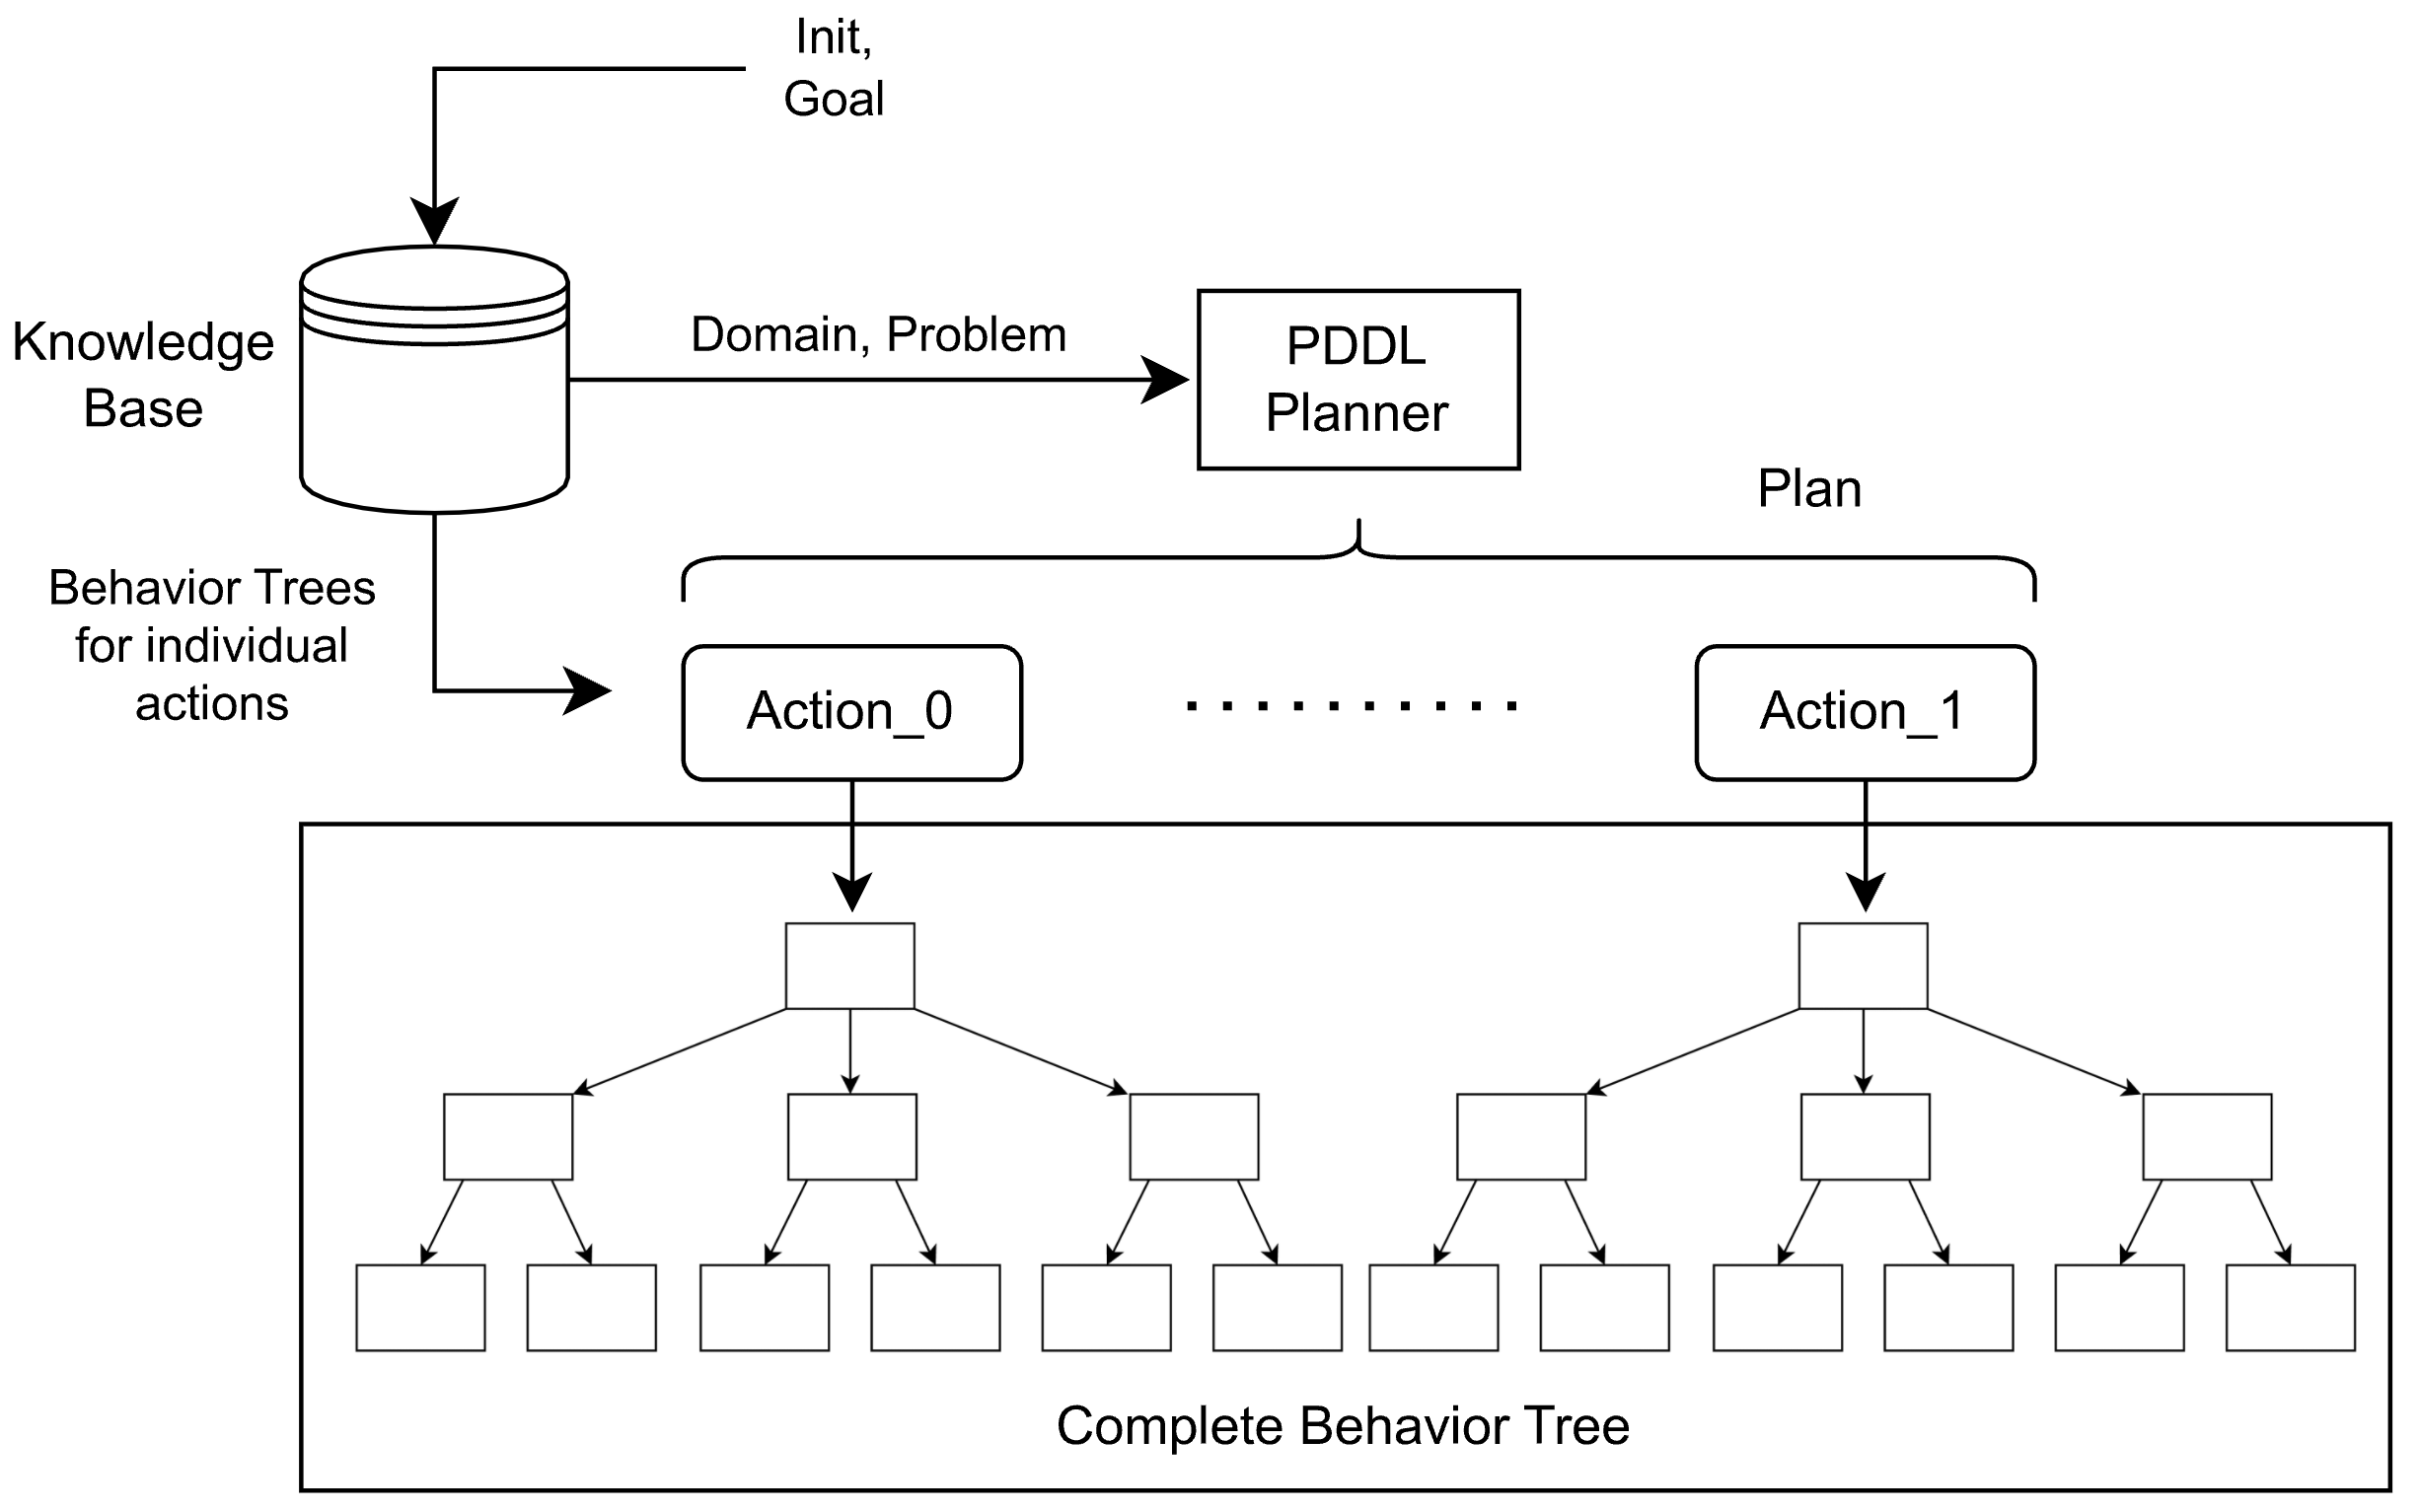
\includegraphics[width=0.9\textwidth]{evaluation_mode.png}
    \caption{Data flow and construction of the behavior tree during evaluation mode.}    
\end{figure}

Apart from the introduction of the new vision system and predicates, the other main modification applied to the pre-existing code was the decision to evaluate the semantic state only at specific instants. Therefore instead of constantly computing the state of the scene, we evaluate it only at the beginning and at the end of each action. The reason for this is the susceptibility of the vision model to false positives for untrained objects. More information on this can be found in section \ref{false_positives_issue}, but essentially in this manner we ensure that the state is evaluated only when the gripper and human operator are outside of the camera's field of view.

Finally, we tested this setup by having it perform the simple assembly task of picking up a button in various positions and inserting it into various different slots on the two button boards.

\begin{figure}[ht]
    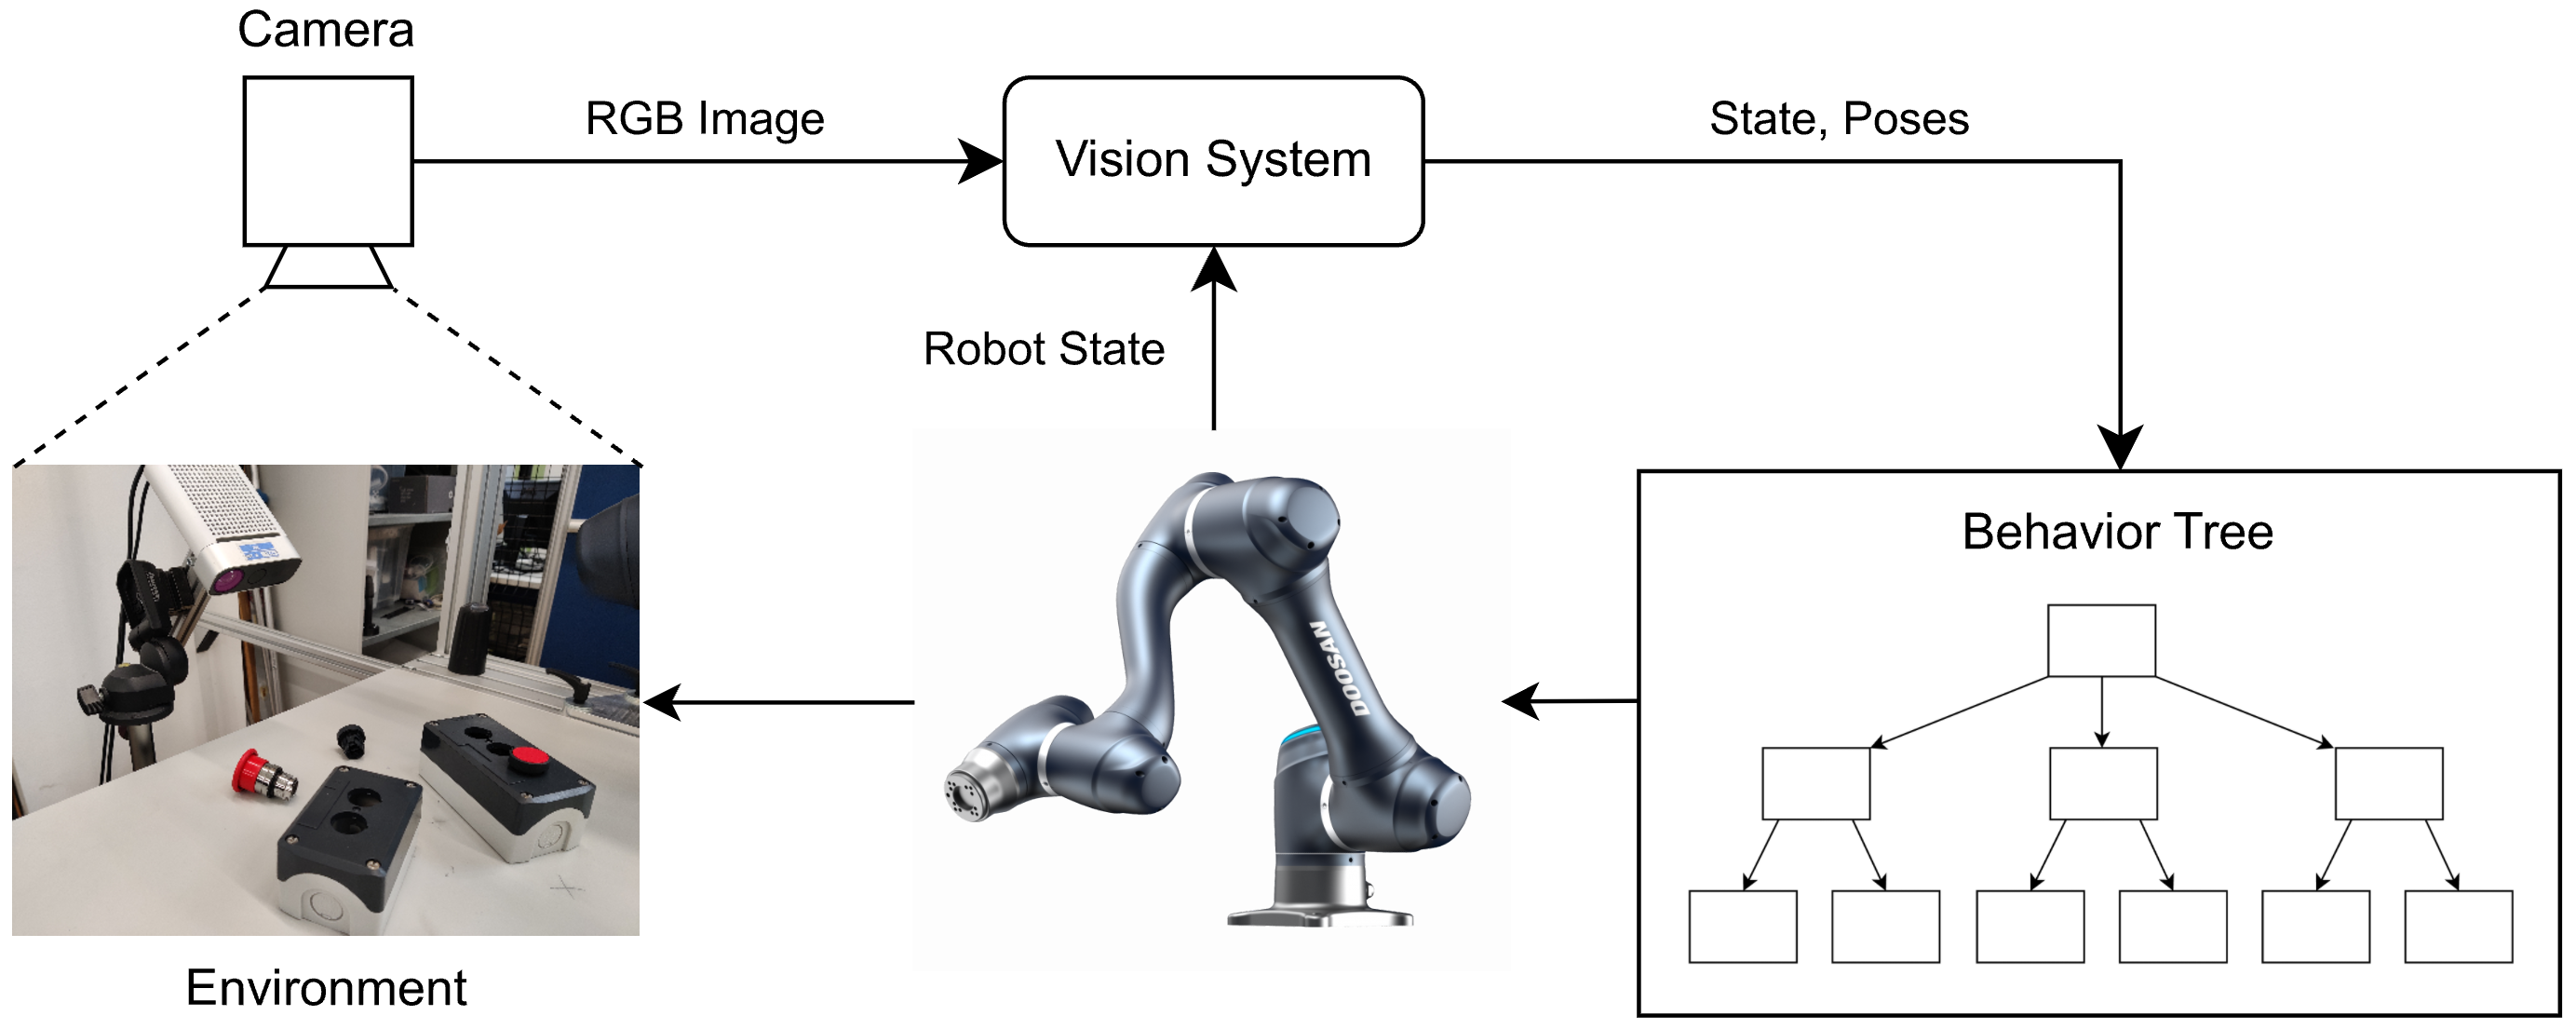
\includegraphics[width=0.8\textwidth]{execute_tree.png}
    \caption{Architecture during execution of the behavior tree.}
\end{figure}

